\documentclass{article}
\usepackage[utf8]{inputenc}
\usepackage{hyperref}
\hypersetup{
    colorlinks=true,
    linkcolor=blue,
    filecolor=blue,      
    urlcolor=blue,
}
\usepackage[a4paper,top=2cm,bottom=2.5cm,left=2cm,right=2cm,marginparwidth=1.75cm]{geometry}
\usepackage{float}
\usepackage{forest}
\usepackage{graphicx}

\title{\textbf{\underline{CSN-232 Reading Assignment-1}}}
\author{
\textbf{Ayush Gupta,19114017} \\
}
\date{3 March 2021}

\begin{document}

\maketitle
\tableofcontents

\section{\underline{Mainframe Systems}}
      \subsection{Introduction}
      Mainframe computers are computers which are used primarily by large organizations for bulk data processing and as servers in large data centers. A mainframe computer is larger and has more processing power than some other classes of computers. \\
      Some vendors of Mainframe Computers are :
      \begin{enumerate}
          \item IBM
          \item Hitachi
          \item Amdahl
          \item Unisys
      \end{enumerate}
      \subsection{Mainframe OS}
      Mainframe Operating Systems are primarily designed to deal with extremely \textbf{high volumes of input and output} and are optimized for \textbf{computational speed}. Moreover since a number of today’s busiest Web sites save their production databases on a mainframe host the OS must be \textbf{robust} and should have less chances of \textbf{total} failure.
      \subsection{Salient features of Mainframe OS}
      \begin{enumerate}
         \item \textbf{High Processing Power and Multi-programming :} Multiprogramming is an essential feature of a Mainframe OS, since speed is the key to it's performance. The OS achieves parallelism by \textbf{minimizing the idle time}, primarily on large I/O operations which consume a more clock cycles as compared to other arithmetic operations,etc.  
      \item \textbf{Spooling :} Spooling stands for \textbf{Simultaneous Peripherals Operations On Line}. It helps implement the principle of \textbf{Multi-programming}. For example, spooling manages printer output by receiving printer output and directing it to a storage device instead of sending it to the printer. When the program finishes, the operating system collects its spooled print output and directs it to the printer.
      \item \textbf{Time Sharing :} Time-sharing is a technique which enables many people, located at various terminals, to use a particular computer at the \textbf{same} time. Time-sharing or multitasking is a logical extension of multiprogramming. Processor's time which is shared among multiple users simultaneously is termed as time-sharing. The main difference between Multiprogrammed Systems and Time Sharing Systems is that in case of Multiprogrammed Systems, the objective is to maximize processor use, whereas in Time-Sharing Systems, the objective is to \textbf{minimize response time}.
      \item \textbf{Virtual Memory :} A technique through which a computer can address more memory than the amount physically installed on the system. This extra memory is actually called virtual memory and it is a section of a hard disk that's set up to \textbf{emulate the computer's RAM}.
      \item \textbf{Batch Processing :} Instead of loading/executing one
      instruction at a time, \textbf{multiple instructions} are loaded (known as batches) for execution.
       \end{enumerate}
       \subsection{Examples of Mainframe Operating System}
       \begin{enumerate}
           \item z/OS
           \item z/TPF (Transaction Processing Facility)
           \item z/VSE (Virtual Storage Extended)
           \item z/VM (Vitual Machine)
           \item Linux for System Z
       \end{enumerate}
       \iffalse
       https://www.wisdomjobs.com/e-university/ibm-mainframe-tutorial-464/characteristic-features-of-mainframe-operating-systems-13539.html
       http://digitalthinkerhelp.com/mainframe-computer-definition-with-their-example-types-and-uses/
       https://en.wikipedia.org/wiki/Mainframe_computer*/
       https://www.ibm.com/support/knowledgecenter/zosbasics/com.ibm.zos.zmainframe/zconc_opsysintro.htm
       
       https://www.guru99.com/operating-system-tutorial.html
       
       https://en.wikipedia.org/wiki/Multiprocessor_system_architecture
       https://ecomputernotes.com/fundamental/disk-operating-system/multiprocessor-operating-system#:~:text=Multiprocessor%20Operating%20System%20refers%20to,memory%20and%20other%20peripheral%20devices.&text=In%20this%20system%20processor%20is%20assigned%20a%20specific%20task.
       https://www.guru99.com/process-synchronization.html#:~:text=Process%20Synchronization%20is%20the%20task,same%20shared%20data%20and%20resources.&text=So%20the%20change%20made%20by,accessed%20the%20same%20shared%20data.
       https://ieeexplore.ieee.org/document/5470386
       http://digitalthinkerhelp.com/what-is-multiprocessor-operating-system-and-its-examples/#:~:text=Examples%20for%20Symmetric%20Multiprocessor%20%E2%80%93%20Windows,%2C%20OS%2F2%20%26%20Linux.
       
       https://blog.stackpath.com/distributed-system/#:~:text=A%20distributed%20system%2C%20also%20known,system%20to%20the%20end%2Duser.
       https://www.geeksforgeeks.org/features-of-distributed-operating-system/
       https://en.wikipedia.org/wiki/Distributed_operating_system#:~:text=A%20distributed%20operating%20system%20is,the%20global%20aggregate%20operating%20system.
       http://digitalthinkerhelp.com/distributed-operating-system-tutorial-with-their-types-examples/
       \fi
    
    \section{\underline{Desktop Systems}}  
    \subsection{Introduction}
     Desktop Systems are the personal computers designed for regular use at a single location on or near a desk or table due to its size and power requirements. They are mainly used for personalized uses, are used by a few individuals and are general purpose computers.
    \subsection{Functionality of Desktop OS}
    \begin{enumerate}
        \item \textbf{Process and memory management :} Process management helps to create and delete a process and also provide mechanisms for \textbf{synchronization and communication} among processes. On the other hand Memory Management helps in efficient allocation of memory resources.
        
        \item \textbf{Security :} Since Desktop Systems are used by individuals who may not have much information about the technical details, they become vulnerable to all sorts of \textbf{malware attacks}, hence security is an important aspect of Desktop Systems.
        
        \item \textbf{Networking Functionality :} It helps the Desktop systems to connect to the world of internet.
        
        \item \textbf{File Management :} It manages all the file-related activities such as organization \textbg{storage, retrieval, naming, sharing, and protection} of files.
        
        \item \textbf{I/O Management :} I/O management routines help abstract the complexities behind the inner working of hardware interaction through device drivers. 
    \end{enumerate}
    \subsection{Examples of some Desktop Systems OS}
     \begin{enumerate}
         \item Windows
         \item Android 
         \item iOS
         \item Mac OS
         \item Linux
         \item Chrome OS
     \end{enumerate}
     \subsection{Market Share}
\begin{figure}[H]
    \centering
    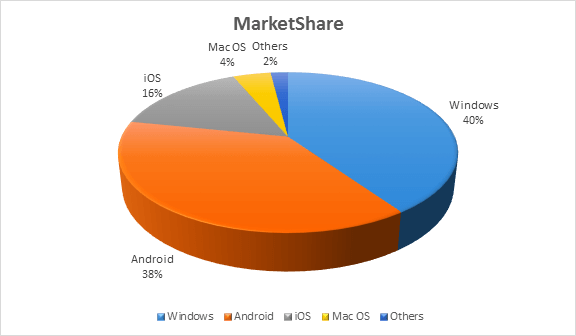
\includegraphics[width=0.95\textwidth]{Market.png}
    \caption{Market Share}
    \label{fig:MarketShare}
\end{figure}
\section{\underline{Multiprocessor Systems}}

\subsection{Introduction}
  Multiprocessor Systems are the systems which have \textbf{more than one processor} working together to complete a task reducing the execution time manifold. The other objectives are fault tolerance and application matching. There are many types of Multiprocessor Systems \textbf{Loosely coupled multiprocessor system, Homogeneous multiprocessor system, Shared memory multiprocessor system}, etc
  
 \subsection{Multiprocessor OS}
  In Multiprocessing OS, the multiple CPUs are in \textbf{close communication} sharing the computer bus, memory and other peripheral devices. Each processor runs an \textbf{identical copy} of operating system and these copies communicate with each other. A master processor controls the system which is a \textbf{master-slave relationship}.
  \subsection{Features of Multiprocessor OS}
Multiprocessor OS is similar to most processor except for the following features.
\begin{enumerate}
    \item \textbf{Process Synchronization :} Since these type of OS have to deal with multiple processors, efficient process synchronization becomes critical. Process Synchronization is the task of coordinating the execution of processes in a way that no two processes can have access to the same \textbf{shared data and resources}. This is important to prevent access of the same data at the same time and to prevent \textbf{data inconsistency}. Data inconsistency occurs when one processor reads the data before other processor has written the data.
    \item \textbf{Resource management :} Resource management is the dynamic allocation and deallocation by an operating system of processor cores, memory pages, and various types of bandwidth to computations that compete for those resources.
    \item \textbf{Scheduling :} The process scheduling is the activity of the process manager that handles the removal of the running process from the CPU and the selection of another process on the basis of a particular strategy.
\end{enumerate}
\subsection{Examples of Multiprocessor OS}
\begin{enumerate}
    \item \textbf{Symmetric Multiprocessor}
    \begin{enumerate}
        \item Windows NT
        \item Solaris
        \item Digital UNIX
    \end{enumerate}
    \item \textbf{Asymmetric Multiprocessor}
    \begin{enumerate}
        \item Sun OS Version 4
        \item IOS
    \end{enumerate}
\end{enumerate}
\section{\underline{Distributed Systems}}
\subsection{Introduction}
A distributed system, also known as distributed computing, is a system with multiple components located on different machines that communicate and coordinate actions in order to appear as a single system to the end-user.
\subsection{Distributed OS}
A distributed operating system is system software over a collection of independent, networked, communicating, and physically computers. They handle jobs which are serviced by multiple CPUs. Each node contains two distinct components.
\begin{enumerate}
    \item The minimal kernel that controls the system hardware.
    \item High level collection of components that coordinate the node's individual and collaborative activities.
\end{enumerate}
These two components work together to provide an illusion that the user is interacting with a single computer which is not the case.
\subsection{Features of Distributed OS}
\begin{enumerate}
    \item \textbf{Transparency :} A distributed system that is capable of presenting itself to users and applications such that it is only a single computer system is called transparent. Moreover, it is an important that the OS hide the fact that the computational resource are distributed across various computers.
    \item \textbf{Reliability :} The central idea behind distributive computing was to minimize the risk of total failures, so even when one node went down, rest of the nodes could be recovered. Reliability is an important factor in distributed OS.
    \item \textbf{Performance :} It should not be the case that the distributed system performs slower than single processor computer because of communication overhead. It is the responsibility of the distributed OS to synchronize the resources for faster execution. 
\end{enumerate}
\subsection{Examples of Distributed OS}
\begin{enumerate}
    \item LOCUS
    \item MICROS
    \item IRIX
    \item DYNIX
    \item AIX
    \item Solaris
    \item Mach
\end{enumerate}
\section{\underline{Clustered Systems}}
\subsection{Introduction}
Clustered Operating Systems resembles parallel operating systems as they possess multiple CPUs. However, a cluster is created when \textbf{two or more computer systems are merged}. Primarily, in a cluster, computers share common storage, and the system works together.

To make a cluster operating system function efficiently, there exists two clusters: hardware and software cluster. A hardware cluster enables \textbf{high-performance disk sharing} between systems, while the software cluster allows all systems to work together.
\begin{figure}[H]
    \centering
    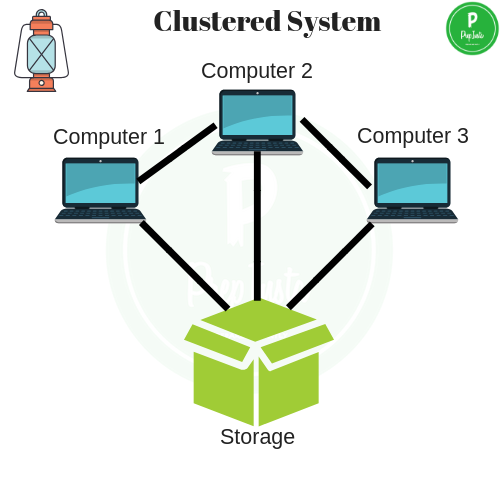
\includegraphics[width=0.75\textwidth]{Clustered.png}
    \caption{Clustered System}
    \label{fig:ClusteredSystem}
\end{figure}
\subsection{Features of Clustered OS}
\begin{enumerate}
    \item \textbf{Mix of Hardware and Software :}
    Cluster Operating systems are mixer of software and hardware clusters. Hardware cluster provides help to share of ultra performance disks in between all computer systems, and Software cluster offers better environment for all system to work together.
    \item \textbf{Scalability :}
    Clustered OS have to be adaptive to addition of new nodes, since addition of new node in a clustered system is relatively easier. 
\end{enumerate}
\subsection{Examples of Clustered OS}
\begin{enumerate}
    \item Oracle Clusterware
\end{enumerate}
\end{document}
